%%%%%%%%%%%%%%%%%%%%%%%%%%%%%%%%%%%%%%%%%
% Maggi Memoir Thesis (WriteLaTeX Version - Compiles with pdflatex)
% XeLaTeX Template
% Version 1.0 (22/12/13)
%
% This template has been downloaded from:
% http://www.LaTeXTemplates.com
%
% Original authors:
% Federico Maggi (fede@maggi.cc) with extensive modifications by:
% Vel (vel@latextemplates.com)
%
% License:
% CC BY-NC-SA 3.0 (http://creativecommons.org/licenses/by-nc-sa/3.0/)
%
% Important note:
% Most of the document content and packages are specified within structure.tex
% so if you need to make modifications to the template have a look there first!
%
%%%%%%%%%%%%%%%%%%%%%%%%%%%%%%%%%%%%%%%%%

%----------------------------------------------------------------------------------------
%   PACKAGES AND OTHER DOCUMENT CONFIGURATIONS
%----------------------------------------------------------------------------------------

\documentclass[11pt,a4paper,twoside]{memoir} % Change font size here (allowable values are 9pt-12pt), change the paper size, specify one or two sided printing and specify whether to show trimming lines

% !TEX root = ./main.tex

%----------------------------------------------------------------------------------------
%	VARIOUS REQUIRED PACKAGES AND CONFIGURATIONS
%----------------------------------------------------------------------------------------

\usepackage[T1]{fontenc} % Support for more character glyphs
\usepackage{lmodern}
\usepackage[superscript,biblabel]{cite}
\usepackage{pdfcomment}
\usepackage[rgb]{xcolor}
%\usepackage[round]{natbib}\citeindextrue % Round brackets around citations, change to square for square brackets
\usepackage{graphicx} % Required to include images
\usepackage{color} % Required for custom colors
\usepackage{amsmath,amssymb,theorem} % Math packages
\usepackage{listings} % Required for including snippets of code
\usepackage{booktabs} % Required for better horizontal rules in tables
\usepackage{xspace} % Provides the ability to use an intelligent space which is used in \institution and \department
\usepackage[printonlyused,withpage]{acronym} % Include a list of acronyms
\usepackage{rotating} % Allows tables and figures to be rotated
\usepackage{hyperref} % Required for links and changing link options
\usepackage{microtype} % Slightly tweak font spacing for aesthetics
\usepackage{pgfplots}
\pgfplotsset{compat=newest} 

\hypersetup{colorlinks, breaklinks, linkcolor=black,citecolor=black,filecolor=black,urlcolor=black} % Set up hyperlinks including colors for references, urls and citations

%\definecolor{c64}{rgb}{.063,0,.612} % Example color definition, the color can be used with the \color{name} command

\makeatletter
\renewcommand{\fnum@figure}{\textsc{\figurename~\thefigure}} % Make the "Figure 1.1" text in small caps
\makeatother

%----------------------------------------------------------------------------------------
%	PAGE LAYOUT
%----------------------------------------------------------------------------------------

% The memoir class used in this template contains the ability to set the stock paper size and the trimmed size independently. It also has the ability to show trim lines showing where stock paper should be trimmed to get the final book size. This can all be a bit confusing so please see the memoir class documentation for more information.

% By default, the paper size is a4paper which is 29.7cm × 21cm. To change this, simply change "a4paper" in the \documentclass[a4paper,...]{memoir} command in thesis.tex to another size such as "letterpaper".
% By default, the trimmed size is 24cm x 17cm and trim lines are shown. To remove trim lines, simply remove "showtrims" from the \documentclass[showtrims,...]{memoir} command in thesis.tex. The size of the trimmed content is set with the \settrimmedsize{}{} command below.
% If you wish to remove trims and set the content to fit the paper size (i.e. no trimming at all), all you have to do is remove "showtrims" as above and comment out the \settrimmedsize{}{} command below.

%\setstocksize{24cm}{17cm} % Uncomment to manually set the stock size and override the setting in \documentclass
%\settrimmedsize{24cm}{17cm}{*} % Change the trimmed area size or comment out this line entirely to fit the content to the paper size without trimming
\setlrmarginsandblock{37.125mm}{*}{0.9} % The first bracket specifies the spine margin, the second the edge margin and the third the ratio of the spine to the edge. Only one or two values are required and the remaining one(s) can be a star (*) to specify it is not needed. By default the edge margin is 10% smaller and 
\setulmarginsandblock{37.125mm}{*}{*} % The first bracket specifies the upper margin, the second the lower margin and the third the ratio of the upper to the lower. Only one or two values are required and the remaining one(s) can be a star (*) to specify it is not needed.
\setmarginnotes{17pt}{51pt}{\onelineskip} % The size of marginal notes, the three values in curly brackets are \marginparsep, \marginparwidth and \marginparpush
\setheadfoot{\onelineskip}{2\onelineskip} % Sets the space available for the header and footer
\setheaderspaces{*}{2\onelineskip}{*} % Sets the spacing above and below the header
\setlength{\trimtop}{0pt} % Sets the spacing above the trimmed area, i.e. moved the trimmed area down the page if positive

% Comment the two lines below to reverse the position of the trimmed content on the stock paper, i.e. odd pages will have content on the right side instead of the left and even pages will have content on the left side instead of the right
\setlength{\trimedge}{\stockwidth}
\addtolength{\trimedge}{-\paperwidth}

\checkandfixthelayout % Makes sure your specifications are correct and implements them in the document

%----------------------------------------------------------------------------------------
%	CHAPTER HEADING STYLE
%----------------------------------------------------------------------------------------

\makeatletter
\makechapterstyle{thesis}{
\renewcommand{\chapternamenum}{}
\setlength{\beforechapskip}{0pt}
\setlength{\midchapskip}{0pt}
\setlength{\afterchapskip}{0pt}
\renewcommand{\chapnamefont}{\LARGE}
\renewcommand{\chapnumfont}{\chapnamefont}
\renewcommand{\chaptitlefont}{\chapnamefont}
\renewcommand{\printchapternum}{}
\renewcommand{\afterchapternum}{}
\renewcommand{\printchaptername}{}
\renewcommand{\afterchaptertitle}{\chapnumfont\hfill\thechapter\\\vspace*{-.3cm}\hrulefill\vspace*{0.5cm}\\}
}
\makeatother

%----------------------------------------------------------------------------------------
%	TABLE OF CONTENTS DEPTH
%----------------------------------------------------------------------------------------

\maxsecnumdepth{subsubsection}
\maxtocdepth{subsection}

%----------------------------------------------------------------------------------------
%	MATH THEOREM DEFINITIONS
%----------------------------------------------------------------------------------------

\theoremstyle{plain}
\newtheorem{thm}{Theorem}[section] % Defines the theorem environment
\newtheorem{prop}[thm]{Proposition} % Defines the proposition environment
\newtheorem{proof}{Proof}[section] % Defines the proof environment
\newtheorem{definition}{Definition}[section] % Defines the definition environment
\newtheorem{example}{Example}[section] % Defines the example environment
\newtheorem{rem}{Remark} % Defines the remark environment
\newtheorem{note}{Note}[section] % Defines the note environment

%----------------------------------------------------------------------------------------
%	CODE SNIPPET CONFIGURATION
%----------------------------------------------------------------------------------------

\lstset{
  basicstyle=\ttfamily\small,
  basewidth=0.55em,
  showstringspaces=false,
  numbers=left,
  numberstyle=\tiny,
  numbersep=2.5pt,
  keywordstyle=\bfseries\ttfamily,
  breaklines=true
}
% Examples of list environments for different programming languages, you will likely need to specify your own
\lstnewenvironment{pseudoc}{\lstset{frame=lines,language=C,mathescape=true}}{}
\lstnewenvironment{logs}{\lstset{frame=lines,basicstyle=\footnotesize\ttfamily,numbers=none}}{}
\lstnewenvironment{cc}{\lstset{frame=lines,language=C}}{}
\lstnewenvironment{c64}{\lstset{backgroundcolor=\color{c64},basewidth=0.65em,basicstyle=\commodoreface\color{c64light},numbers=none,framerule=10pt,rulecolor=\color{c64light},frame=tb,framexbottommargin=30pt}}{}
\lstnewenvironment{html}{\lstset{frame=lines,language=html,numbers=none}}{}
\lstnewenvironment{pseudo}{\lstset{frame=lines,mathescape=true,morekeywords={learn_string_domain, save_model}}}{}
\lstnewenvironment{pseudoctiny}{\lstset{language=C,mathescape=true,basicstyle=\tiny\sffamily}}{}
\lstnewenvironment{cctiny}{\lstset{language=C,basicstyle=\tiny\sffamily}}{}
\lstnewenvironment{pseudotiny}{\lstset{mathescape=true,basicstyle=\tiny\sffamily}}{} % Include the file containing the code defining the structure and style of the document
%------------------------------------------------
% Fonts

\renewcommand*{\acffont}[1]{{\normalsize\itshape #1}} % Font style for the acronym text (e.g. Do It Yourself)
\renewcommand*{\acfsfont}[1]{{\normalsize\upshape #1}} % Font style for the acronym in bracket (e.g. (DIY))

%------------------------------------------------
% Hyphenations

\hyphenation{a-no-ma-lous a-no-ma-ly amounts breaches} % Specify custom hyphenation points in words with dashes where you would like hyphenation to occur, or alternatively, don't put any dashes in a word to stop hyphenation altogether

%----------------------------------------------------------------------------------------
%   TITLE PAGE
%----------------------------------------------------------------------------------------
%----------------------------------------------------------------------------------------

\makeindex % Write an index file

\begin{document}

%
\begin{titlepage}
                % \newgeometry{top=25mm,bottom=25mm,left=38mm,right=32mm}
                \setlength{\parindent}{0pt}
                \setlength{\parskip}{0pt}
                % \fontfamily{phv}\selectfont

                {
                                \Large
                                \raggedright
                                Imperial College London\\[17pt]
                                Department of Electrical and Electronic Engineering\\[17pt]
                                Final Year Project Report 2015\\[17pt]
 
                }

                \rule{\columnwidth}{3pt}
                \vfill
                \centering
                  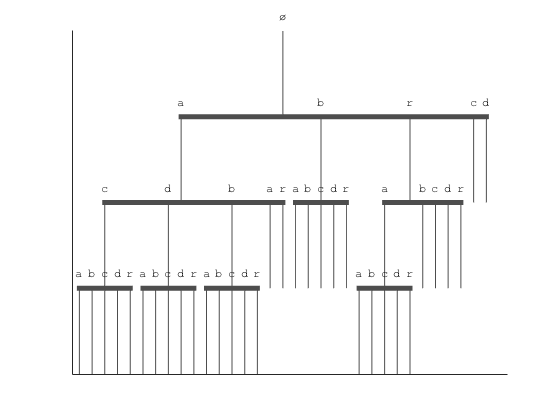
\includegraphics[width=0.7\columnwidth,height=60mm,keepaspectratio]{background/cover.png}
                \vfillba
                \setlength{\tabcolsep}{0pt}

                \begin{tabular}{p{40mm}p{\dimexpr\columnwidth-40mm}}
                                Project Title: & \textbf{Proactive Multimedia Caching} \\[12pt]
                                Student: & \textbf{Leon Zhang} \\[12pt]
                                CID: & \textbf{00683680} \\[12pt]
                                Course: & \textbf{EEE4} \\[12pt]
                                Project Supervisor: & \textbf{Dr. Deniz Gunduz} \\[12pt]
                                Second Marker: & \textbf{Dr T.K. Kim} \\
                \end{tabular}


\end{titlepage}

\begin{titlingpage}
                % \newgeometry{top=25mm,bottom=25mm,left=38mm,right=32mm}
                \setlength{\parindent}{0pt}
                \setlength{\parskip}{0pt}
                % \fontfamily{phv}\selectfont

                {
                                \Large
                                \raggedright
                                Imperial College London\\[17pt]
                                Department of Electrical and Electronic Engineering\\[17pt]
                                Final Year Project Report 2014\\[17pt]
 
                }

                \rule{\columnwidth}{3pt}
                \vfill
                \centering
                  %\includegraphics[width=0.9\columnwidth,height=90mm,keepaspectratio]{titlegraph.png}
                \vfill
                \setlength{\tabcolsep}{0pt}

                \begin{tabular}{p{40mm}p{\dimexpr\columnwidth-40mm}}
                                Project Title: & \textbf{Simulator for Decentralised Energy Systems} \\[12pt]
                                Student: & \textbf{Yuchen Wang} \\[12pt]
                                CID: & \textbf{00683700} \\[12pt]
                                Course: & \textbf{EE4 (EM)} \\[12pt]
                                Project Supervisor: & \textbf{Dr. Jeremy V. Pitt} \\[12pt]
                                Second Marker: & \textbf{Dr. Javier A. Barria} \\
                \end{tabular}
\end{titlingpage}


\frontmatter % Use roman page numbering style (i, ii, iii, iv...) for the pre-content pages

%----------------------------------------------------------------------------------------
%   PREFACE
%----------------------------------------------------------------------------------------

\section*{Acknowledgements}
I would like to thank my supervisor Dr Jeremy Pitt for taking the time to impart advice, guidance and supervision over the past academic year on this project. \\ 
I would like to thank e.quinox, all members past, present for giving me the opportunity of a lifetime and giving me the information to make this project relevant. \\
I would also like to thank my friends, housemates and fellow colleagues who have made my last 4 years the best experience it could possibly be. \\
Finally, I would like to thank my family, in particular my mother for their support and love.

\begin{flushright}
%\textsc{\theauthor}\\
Yuchen Wang\\
June 2015
\end{flushright}

\cleartoverso % Force a break to an even page

%----------------------------------------------------------------------------------------
%   ABSTRACT
%----------------------------------------------------------------------------------------

\begin{abstract}

In many developing countries the electricity grid network is underdeveloped, causing low levels of rural electrification. However, electricity access in these rural communities are not non-existent. There are a number isolated and independent electricity generators owned by individuals, NGOs and local government institutions. This project explores the feasibility of a Decentralised Community Energy System which utilises these isolated sources of electricity to create a community micro grid. It is planned to conduct the feasibility study with the help of a simulation to be developed using Presage2 and Java. This report outlines the deliverables, planning process, background research, and the design and implementation of the simulation model. 

\end{abstract}

\cleartoverso % Force a break to an even page


%----------------------------------------------------------------------------------------
%   TABLE OF CONTENTS
%----------------------------------------------------------------------------------------

\tableofcontents* % Print the table of contents

\cleartoverso % Force a break to an even page

%----------------------------------------------------------------------------------------
%   LIST OF FIGURES
%----------------------------------------------------------------------------------------

\listoffigures % Print the list of figures

\cleartoverso % Force a break to an even page

%----------------------------------------------------------------------------------------
%   LIST OF TABLES
%----------------------------------------------------------------------------------------

\listoftables % Print the list of tables

\cleartoverso % Force a break to an even page

%----------------------------------------------------------------------------------------
%   ACRONYMS
%----------------------------------------------------------------------------------------

\chapter{List of Acronyms}
\begin{acronym}\addtolength{\itemsep}{-\baselineskip}
  \acro{AIC}{Akaike Information Criterion}
  \acro{ARMA}{Auto Regressive Moving Average}
  \acro{ARMAX}{Auto Regressive Moving Average eXogenous}
  \acro{ARX}{Auto Regressive eXogenous}
  \acro{AR}{Auto Regressive}
  \acro{ARR}{Alert Reduction Rate}
  \acro{ANSI}{American National Standard Institute}
  \acro{ASCII}{American Standard for Information Interxchange}
  \acro{BIC}{Bayesian Information Criterion}
  \acro{BMU}{Best Matching Unit}
  \acro{BSM}{Basic Security Module}
  \acro{CDF}{Cumulative Density Function}
  \acro{CDX}{Cyber Defense eXercise}
  \acro{CIA}{Confidentially Integrity Availability}
  \acro{CIDS}{Collaborative IDS}
  \acro{CPU}{Central Processing Unit}
  \acro{CSV}{Comma Separated Values}
  \acro{CTF}{Capture The Flag}
  \acro{DAG}{Direct Acyclic Graph}
  \acro{DARPA}{Defense Advanced Research Projects Agency}
  \acro{DB}{DataBase}
  \acro{DBMS}{DataBase Management System}
  \acro{DIDS}{Distributed IDS}
  \acro{DNS}{Domain Name System}
  \acro{DOM}{Document Object Model}
  \acro{DoS}{Denial of Service}
  \acro{DR}{Detection Rate}
  \acro{DTD}{Document Type Definition}
  \acro{ED}{Elementary Detector}
  \acro{ELF}{Executable Linux Format}
  \acro{FN}{False Negative}
  \acro{FNR}{False Negative Rate}
  \acro{FPR}{False Positive Rate}
  \acro{FP}{False Positive}
  \acro{FSA}{Finite State Automaton}
  \acro{FTP}{File Transfer Protocol}
  \acro{GCI}{Granger Causality Index}
  \acro{GCT}{Granger Causality Test}
  \acro{HIDS}{Host-based Intrusion Detection System}
  \acro{HMM}{Hidden Markov Model}
  \acro{HTML}{HyperText Markup Language}
  \acro{HTTP}{HyperText Transfer Protocol}
  \acro{ICD}{Idealized Character Distribution}
  \acro{IDEVAL}{Intrusion Detection eVALuation}
  \acro{IDMEF}{Intrusion Detection Message Exchange Format}
  \acro{IDS}{Intrusion Detection System}
  \acro{IDWG}{Intrusion Detection Working Group}
  \acro{ID}{Intrusion Detection}
  \acro{IETF}{Internet Engineering Task Force}
  \acro{IODEF}{Incident Object Description and Interchange Format}
  \acro{IPS}{Intrusion Protection System}
  \acro{ISP}{Internet Service Provider}
  \acro{IP}{Internet Protocol}
  \acro{IR}{Information Retrieval}
  \acro{IRC}{Internet Relay Chat}
  \acro{ISS}{Internet Security Systems}
  \acro{JSON}{JavaScript Object Notation}
  \acro{KBS}{Knowledge Base System}
  \acro{KS}{Kolmogorov-Smirnoff}
  \acro{LARIAT}{Lincoln Adaptable Real-time Information Assurance Testbed}
  \acro{LERAD}{Learning Rules for Anomaly Detection}
  \acro{LL}{Lincoln Laboratory}
  \acro{MDL}{Minimum Description Length}
  \acro{MIT}{Massachusetts Institute of Technology}
  \acro{ML}{Maximum Likelihood}
  \acro{MTU}{Maximum Transfer Unit}
  \acro{NIDES}{Next-generation Intrusion Detection Expert System}
  \acro{NIDS}{Network-based Intrusion Detection System}
  \acro{NNID}{Neural Network Intrusion Detection}
  \acro{NSTISSC}{National Security Telecomm. and Information Systems Sec. Committee}
  \acro{NTP}{Network Time Protocol}
  \acro{PC}{Program Counter}
  \acro{PDF}{Probability Density Function}
  \acro{PHAD}{Packet Header Anomaly Detection}
  \acro{PHP}{PHP Hypertext Preprocessor}
  \acro{PID}{Process IDentifier}
  \acro{ROC}{Receiving Operating Characteristic}
  \acro{SADE}{Syscall Sequence Arguments Anomaly Detection Engine}
  \acro{SDEE}{Security Device Event Exchange}
  \acro{SMTP}{Simple Message Transfer Protocol}
  \acro{SOM}{Self Organizing Map}
  \acro{SQL}{Structured Query Language}  
  \acro{SRI}{Stanford Research Institute}
  \acro{SSH}{Secure SHell}
  \acro{STATL}{State Transition Analysis Technique Language}
  \acro{SVN}{SubVersioN}
  \acro{SYN}{SYNchronize}
  \acro{TCP}{Trasmission Control Protocol}
  \acro{TF}{Truth File}
  \acro{TN}{True Negative}
  \acro{TNR}{True Negative Rate}
  \acro{TOS}{Type Of Service}
  \acro{TP}{True Positive}
  \acro{TTL}{Time To Live}
  \acro{UCSB}{University of California Santa Barbara}
  \acro{ULISSE}{Unsupervised Learning IDS with 2-Stages Engine}
  \acro{UDP}{User Datagram Protocol}
  \acro{UML}{Unified Modeling Language}
  \acro{URL}{Uniform Resource Locator}
  \acro{VPN}{Virtual Private Network}
  \acro{XML}{eXtensible Markup Language}
  \acro{XSD}{XML Schema Definition}
  \acro{XSS}{Cross-Site Scripting}
\end{acronym} % Include a List of Acronyms section using acronyms.tex where they are defined

%\cleartoverso % Force a break to an even page

%----------------------------------------------------------------------------------------
%   COLOPHON
%----------------------------------------------------------------------------------------

% \thispagestyle{empty} % Remove all headers and footers from this page

% \vspace*{2em}
% \renewcommand{\abstractname}{Colophon}
% \begin{abstract}
% This document was typeset using the \textsf{XeTeX} typesetting system created by the Non-Roman Script Initiative and the memoir class created by Peter Wilson. The body text is set 10pt with~Adobe Caslon Pro. Other fonts include \texttt{Envy Code R}, \textsf{Optima Regular} and. Most of the drawings are typeset using the \textsf{TikZ/PGF} packages by Till Tantau.
% \end{abstract}
% \vfill

%----------------------------------------------------------------------------------------
%   CONTENT CHAPTERS
%----------------------------------------------------------------------------------------

\mainmatter % Begin numeric (1,2,3...) page numbering

\chapterstyle{thesis} % Change the style of the Chapter header to that defined in structure.tex

\pagestyle{Ruled} % Include the chapter/section in the header along with a horizontal rule underneath

% !TEX root = ../main.tex
\chapter{Introduction}
\label{introduction}

In many areas of rural developing countries, there are often no wide-spread access to a continuous and reliable electricity supply such provided by the country's electricity grid \cite{IEA-web:2015}. However there exists many isolated sources of electricity generation such as solar panels and standalone diesel generators utilised by relatively wealthy households, shops and buildings belonging to large organisations. 

The aim of this project is to explore the idea of using a holonic institution to model a Decentralised Community Energy System which bring together the existing decentralised generation infrastructure to provide an affordable source of reliable electricity for users in rural communities. 

Over the course of this project, a multi-agent simulation model was built using Presage2 with individual households and businesses modelled agents. The agents can be grouped together to form communities such as villages, which in turn can be grouped together to form a larger entity such as a district or a province. 

%To do: cite here:
With humans being social creatures who are likely to band together to form communities, the structure of the decentralised energy system model will be designed in a similar way with holonics. The structure of how the simulation is designed is based on the design of holonic systems. In the case of this project, the simulation will be to distribute fairly electrical power between interrelated agents which are in turn composed of interrelated subagents recursively, until reaching lowest level of subagents (households and businesses). 

To allow the model to be realistic, candidate rural communities with no access to a source of reliable electricity will be identified using data and research. Additional data on usage habits and potential generation profiles of generators in the candidate areas will be obtained through research to produce a simulation model that is accurate and relevant.

Include:
\begin{itemize}
\item Design Choices: Holonics, design of objectives
\item difficulties and how they were designed:
\subitem Out of order parallel execution
\subitem Presage
\subitem One action per time step
\item Discovery or invetion of something novel?
\item What did you learn:
\subitem Java, Presage, Software design
\end{itemize}


This report outlines the design, implementation and testing of a holonic multiagent simulation of a decentralised energy system. 
 % Include the introduction chapter
% !TEX root = ../main.tex
\chapter{2. Background}
\label{Background}

\section*{Electricity as a Common Pool Resource}
A Common Pool Resource is a depletable resource which can be utilised by a group of people, characterised by a reduction in the availability of this resource as individuals withdraw or utilise this resource \cite{Ostrom:90}.  Electricity can be a Common Pool Resource if there exists a finite amount of electricity generation capacity. As users connect demand appliances to the generators, the availability of electricity supply for additional demand diminishes.

In developing communities with significant generation from renewable sources such as wind and solar, the availability of power is subject to variation between periods in time. This inherent volatility in the amount of available resource could increase the likelihood of selfish actions of by individuals in the community.

Ostrom showed that Common Property Regimes can be formed to maintain the Common Pool Resources by controlling the access to the resource \cite{Ostrom:90}. 

\section*{Decentralised Community Energy Systems as a Holonic System}
A holonic system (or holarchy) is a system which is composed of interrelated subsystems or institution, each of which are in turn composed of sub-subsystems  or institution and so on, recursively until reaching a lowest level of "elementary" subsystems. Each system, sub-system or institution has a well-defined set of goals or objectives which is achieved through enforcing a set of rules on its members (subsystems, sub-institutions and elementary entities)\cite{Pitt:Holonic_Institutions}. It is this type of Common Property Regime that will be explored in this project to maintain the Common Pool Resource that is electricity. 

In the context of a rural Decentralised Community Energy system, a network between households, communities and even villages to pool and share electricity as a common pool resource can be modelled as a holonic system. The holonic system in this case would be composed of communities such as Districts, Provinces, Sectors which are composed of sub-communities such as Towns and Villages. The sub-communities would be composed of many "elementary" subsystems such as households, businesses and other points of connection for electricity. Each community or institution has the goal of fairly allocating electricity to all members. This goal would be achieved with the assumption that they are provided with the necessary infrastructure and powers for enforcing quotas and contribute to a common pool of electricity.

\section*{Ostrom's principles}

\section*{Distributive Justice and Fair Allocation}
Given that the necessary infrastructure and powers exist for enforcing quotas and contribution to the Common Pool, the allocation needs to be fair. Being fair forms two of the necessary Ostrom's Principles for Enduring Institutions in a Common Property Regime \cite{Ostrom:90}. \\

Rescher's Canon of Distributive Justice

\subsection*{Multi-Agent Simulation}
The simulation will be designed as a Multi-Agent System (MAS). MASes are particularly suited for this kind of model as Agents in MASes have three very important characteristics:
\begin{itemize}
	\item Autonomous: Agents act independently
	\item Local view: no Agent can see or manipulate the environment it is in
	\item Decentralised: There is no Agent which controls the action of all Agents
\end{itemize}
In reality, individual households which are represented by Agents in the simulator all perform actions according to their individual and unique needs, and not controlled by a third party. This makes Autonomy and Decentralisation a requirement for the Agents in the Simulator. Participants or households connected to the network can't directly control how other participants use or generate electricity for the Common Resource Pool, making it an requirement for the Agent to have a Localised view. 

\subsection*{About Presage 2}
Presage 2 is a simulation platform for multi-nodal or Agent simulation of societies. The platform was built by Sam Macbeth and is currently maintained by PhD students within Imperial. This platform was chosen for the simulator as it enables the investigation of the impact of agent design (such as household behaviour), network properties (constraints on access) and the physical environment on individual agent behaviour and long-term global network performance \cite{Presage2-Desc:2015}. In the context of this Project, each Node/Agent can represent individuals, households, businesses or generators. 

Presage 2 was chosen for this project as it is a platform which allows the rapid prototyping of complex Agent societies. Presage 2 Agents are only allowed to act during increments of time steps, which makes the simulation a discrete time driven one. Figures \ref{fig:Presage_architecture} and \ref{fig:Presage_sim_architecture} illustrates general and simulation archtecture.

\begin{figure}[h!]
	\centering
	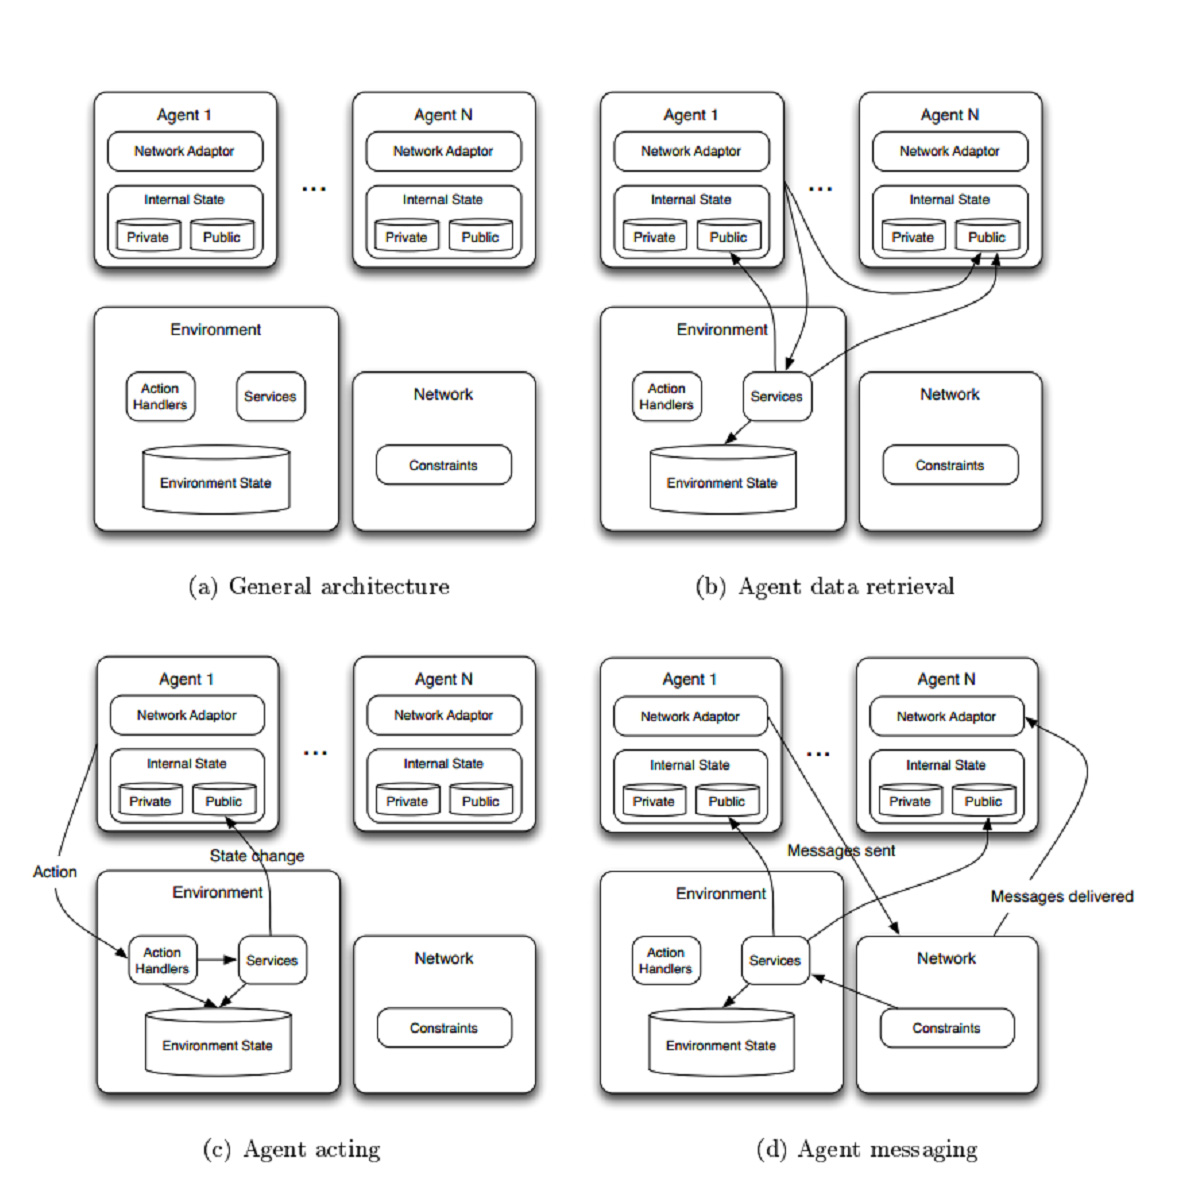
\includegraphics[scale=0.25]{Images/Presage.jpg}
	\caption{Presage 2 architecture \cite{Presage_Kyoto:2015}}
	\label{fig:Presage_architecture}
\end{figure}

\begin{figure}[h!]
	\centering
	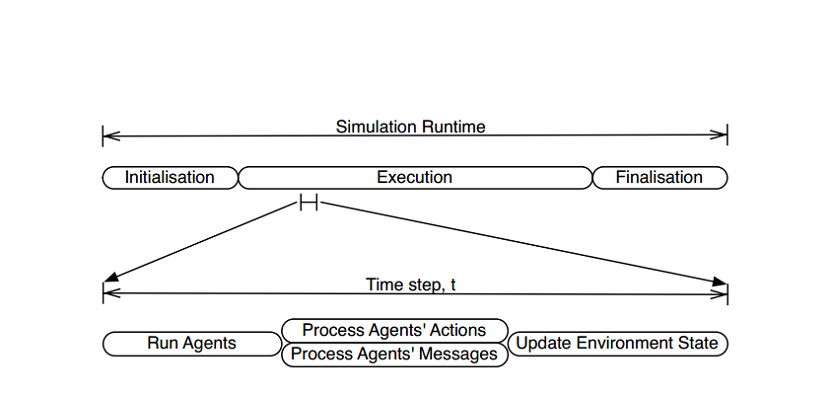
\includegraphics[scale=0.4]{Images/Presage2.jpg}
	\caption{Presage 2 simulation architecture \cite{Presage_Kyoto:2015}}
	\label{fig:Presage_sim_architecture}
\end{figure}

\clearpage

\section*{Rural Communities in Rwanda}
With an estimated 25\% rural electrification rate in 2009 \cite{IEA-web:2015}, rural Africa is one obvious candidate for simulation scenarios. Vast amounts of rural communities remain un-electrified. For a realistic simulation scenario, knowledge of existing infrastructure in place will need to be obtained. With many areas within many countries in Africa, Rwanda in particular has been identified as a good potential simulation scenario to research. Data is difficult to source for rural communities in developing countries, however in the case of Rwanda, some data can be easily from the student society e.quinox. e.quinox is a student-led society which aims to find a scalable solution for rural electrification who mainly operate in Rwanda \cite{e.quinox-web:2015}. The subsections below outline some of the ways remote rural communities are able to access electricity in Rwanda.

\subsection*{Electricity Generation}
One of the solutions currently being implemented by e.quinox is the "Energy Kisok" model \cite{e.quinox-EK-web:2015}. The "Energy Kiosk" model features an Energy Kiosk - a building where the generation, storage and distribution of electricity takes place.
In e.quinox operated kiosks, electricity is generated from renewable sources.
Traditionally, this has been with solar panels. However, hydro-electric generation has been demonstrated to be feasible with the recent construction of a "Hydro Kiosk" at Rugaragara Falls in Southern Rwanda.

\subsection*{Storage and Distribution}
Within each kiosk, electricity that is generated is stored in storage batteries placed in the kiosks. The storage batteries regulate power output and allows access to electricity in the kiosk even during periods of no electricity generation.

\subsubsection*{Battery Box}
In the absence of any electricity distribution infrastructure, e.quinox has traditionally provided a number of portable batteries for the purpose of electricity distribution. An example of the portable batteries can be seen in Figure \ref{fig:AmaziBox}.

\begin{figure}[h!]
\centering
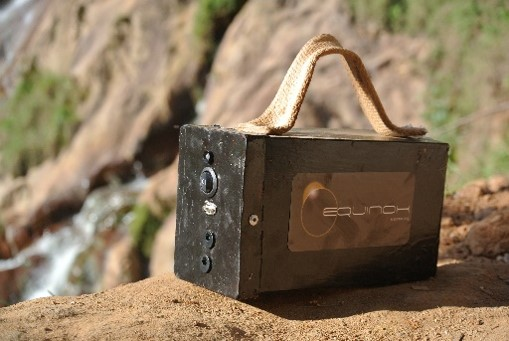
\includegraphics[scale=0.7]{Images/AmaziBox.jpg}
\caption{First Generation e.quinox Battery Boxes deployed at Rugaragara Falls Kiosk}
\label{fig:AmaziBox}
\end{figure}

Consumers from local community pay to hire the battery boxes under one of two payment schemes: pay-per-recharge and pay-per-month \cite{e.quinox-Hydro-web:2012}. The biggest difference between the two schemes are that users can recharge as often as they would like with pay-per-month. Both payment schemes involve the recharge of the boxes at the energy kiosk when they are depleted of energy.

A potential use case of this project can be the simulation of charging of battery boxes at an energy kiosk. This could alleviate congestion and improve asset utilisation of the existing distribution systems by reducing the turn-around time of battery boxes for customers.

\subsubsection*{Micro Grid}
With the recent completion of a hydro-electric kiosk. e.quinox for the first time has a kiosk with access to an always-on generator. With a limited number of battery boxes in circulation and a constant generation available during the off-peak hours, there is excess capacity for electricity generation.

To improve utilisation of the generator in the kiosk, e.quinox has recently started conducting a feasibility study into constructing a transmission line and a distribution network which will serve a village near the kiosk with a view to make the most of the electricity generated.

Preliminary surveys conducted in the nearest village to the kiosk indicates the demand could exceed the amount of excess power generated by the kiosk. 

The result of this project can be used in conjunction with e.quinox to conduct the feasibility study of implementing the Micro-Grid. Should a trading platform for energy also be built, the Micro-Grid could serve as a test-bed for this new system.

\subsubsection*{Standalone Solution}
The Standalone Solution is an independent electrification solution which was recently developed by e.quinox for customers who live far from energy kiosks.

The Stand-alone solution consists of a pay-as-you-go solar electricity generation and storage kit, known as the Izuba.Box \cite{e.quinox-Standalone-web:2012}.  With the Izuba.Box, customers no longer have to travel regularly back to the Energy Kiosk for electricity. Solar panels are installed on the customer’s roof, and is connected to a sealed box which contains a large battery box. The attached large battery box allows a regulated power output and access to electricity during dark hours. 

With the customers not returning to Energy Kiosks, the battery boxes are not hired out like the battery boxes are. The high capital costs of the independent solar system is spread over typically a two year rent-to-own payment plan using a mobile payment system.

It is hoped that the Standalone Solution and additional generation from the Energy Kiosk can be complemented the battery boxes in circulation to provide a continuous access to electricity to all households in the village.

\clearpage

\begin{figure}[h!]
\centering
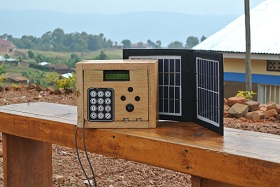
\includegraphics[scale=3]{Images/standalone_box.jpg}
\caption{First Generation Izuba.Box deplyed in Minazi, Northern Rwanda}
\label{fig:IzubaBox}
\end{figure}

\subsection*{Rugaragara Falls as a Simulation Scenario}
In developing countries such as Rwanda, poor communities with no access to grid electricity are often in isolated locations such as Rugaragara Falls. The local District Sector office estimates Grid Access won't be available before 2020. In these areas, access is often difficult, making fuel for generators often difficult to obtain. Therefore, locals often depend on other available sources of electricity such as solar and wind power. However, these methods of generation provides highly variable amounts of energy which depends on other variables such as weather. Without access to redundancies received from the national electricity grid to ensure continual access to electricty, it can be beneficial for prosumers within these areas to form a micro-grid, which in many cases would be cheaper than connecting to the national grid. %As an example, many people still choose to use battery boxes provided by e.quinox, which is cheaper than connecting to the grid.

% \subsection{Additional Research}
% e.quinox in Rwanda only presents us with one scenario. Additional research is required for other regions such as South America and the Indian Subcontinent to look at potential new scenarios and use cases for various generators and electrical appliances.

% The information above only outlines the existing infrastructures in place. Additional work needs to be done to obtain relevant usage data from e.quinox customers and other electricity users to accurately build a relevant generation mix and demand model.

% In some regions such as Minazi, e.quinox provides the only source of accessible electricity for the local populace. Data on their usage should be more readily available than some of the other locations in other countries. 
% !TEX root = ./main.tex
\chapter{Requirements}
\label{Requirements}

It is therefore required that the simulation platform will have the following features:
\begin{itemize}
  \item Multiple Forms of Generation: Renewable and Non-renewable generators which can operate continuously or discontinuously
  \item Realistic Generator Models: Programmable variable generation power output to simulate wind and solar power
  \item Multiple demand centres: the simulation will be of one or more communities operating with a number of households/businesses requiring electricity
  \item Self organising by the system to appropriate the available power fairly to all users
\end{itemize}

As this is a simulation to be implemented in Presage2, there are no specific requirements which must be adhered to with regards to speed, portability and performance.  

The simulation is to be developed using Presage2. It is hoped that a network of Decentralised Community Energy Systems can be simulated, and a working trading system can also be developed for the trading of limited available energy within communities towards the end of the project time frame. 
% !TEX root = ./main.tex
\chapter{Planning}
\label{Planning}
Following a number of supervisor meetings with Dr Pitt, a number of work items have been identified. A Gantt Chart was created to facilitate the planning and tracking of the project progress. A copy of the current Gantt Chart can be seen in Figure \ref{fig:GanttChart}. The Gantt Chart was a continuous working document which will be update as the project progresses. Tasks were added as new ideas for the project became available. 

\begin{figure}[h!]
\centering
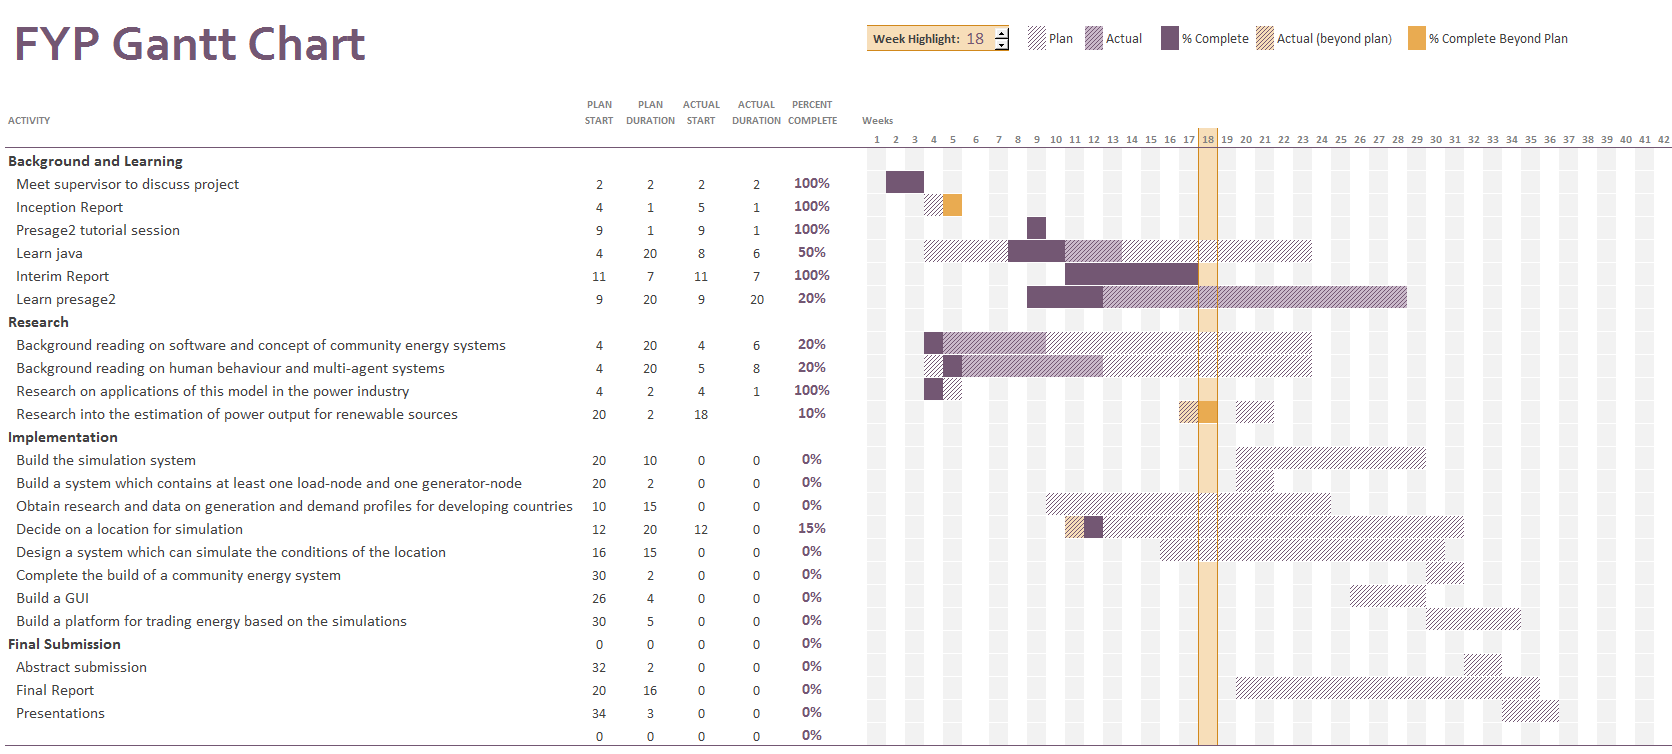
\includegraphics[scale=0.5, angle=90]{Images/GanttChart.png}
\caption{Up to date Gantt chart}
\label{fig:GanttChart}
\end{figure}
% !TEX root = ../main.tex
\chapter{Analysis and Design}
\label{analysis}



% !TEX root = ../main.tex
\chapter{Implementation}
\label{Implementation}
In this section, how the design is implemented will be described in detail

\section*{Agents}
Agents in Presage 2 are created by extending the AbstractParticipant class. As Virtual Agents and Prosumer Agents behave in a similar fashion, the Prosumer Agent is designed to extend the Virtual Agent with additional properties such as ParentID and ability to add Demand/Generation profiles.

\begin{figure}[!h]
	\centering
	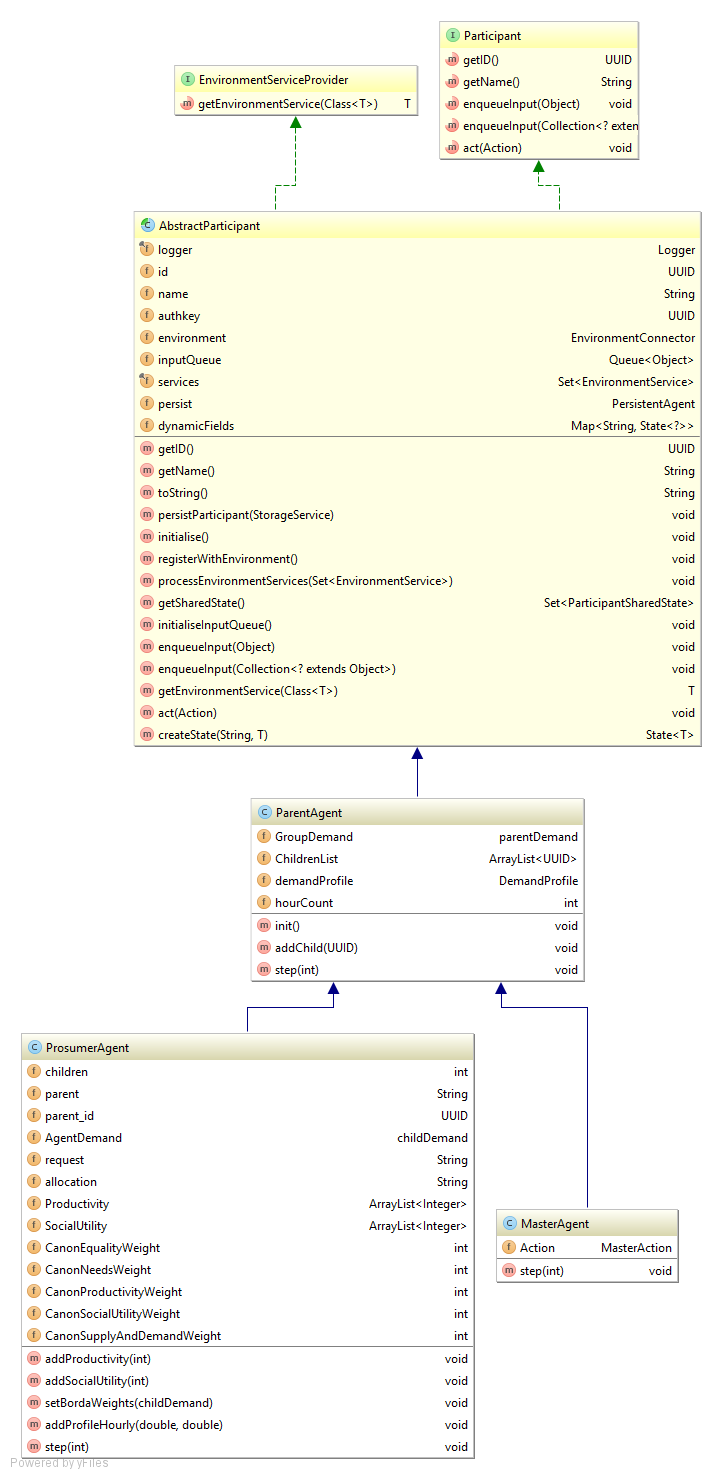
\includegraphics[scale=0.71]{Images/AgentUML.png}
	\caption{Agent UML Diagram}
	\label{fig:AgentUML}
\end{figure}

\section*{Environment Services}
All Agents act within Environments, which would contain shared state between Agents. In the context of this simulation shared state would be information such as the amount available in the Common Resource Pool.

\begin{figure}[!h]
	\centering
	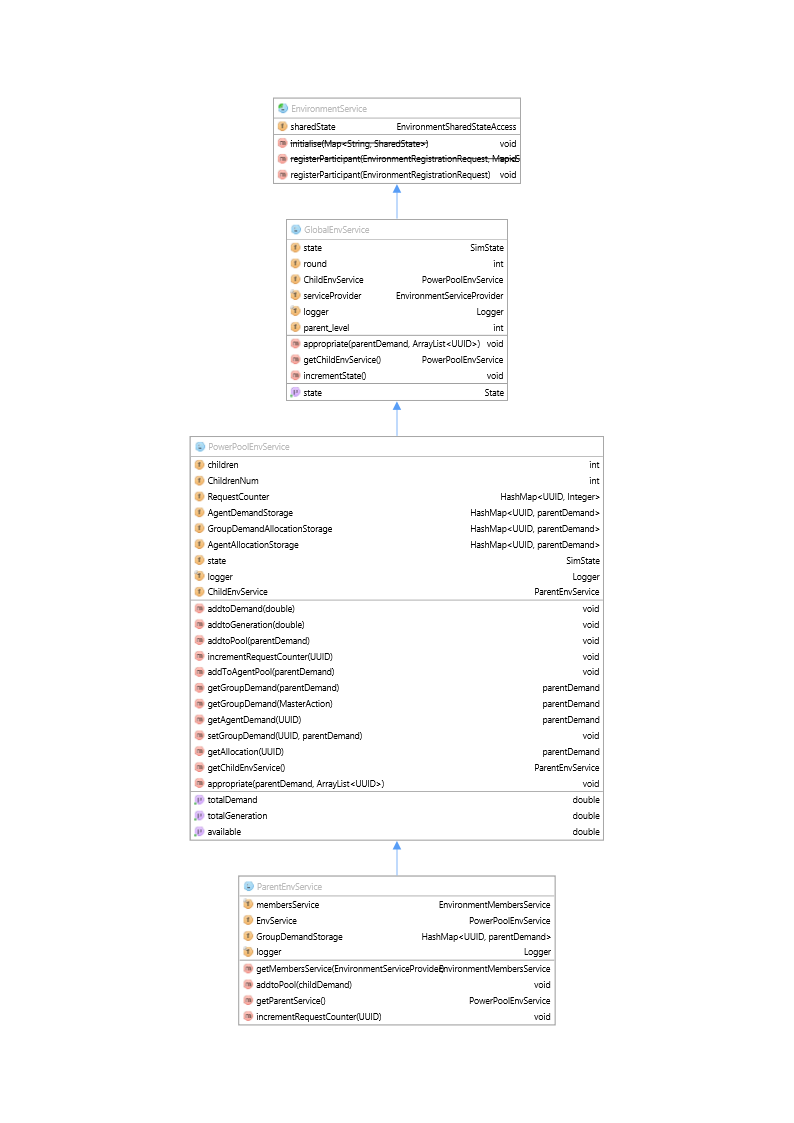
\includegraphics[scale=0.71]{Images/EnvironmentUML.png}
	\caption{Environment Services UML Diagram}
	\label{fig:ServiceUML}
\end{figure}

\subsection*{Action}
To act on the Environment or acess a shared state in the Environment, Agents are expected to perform an Action. In the context of this simulation, Action would be Demand/Generation requests. As Generation can be modelled as a negative Demand, a single Action can be defined to allow the contribution and appropriation of electricity. 

\begin{figure}[!h]
	\centering
	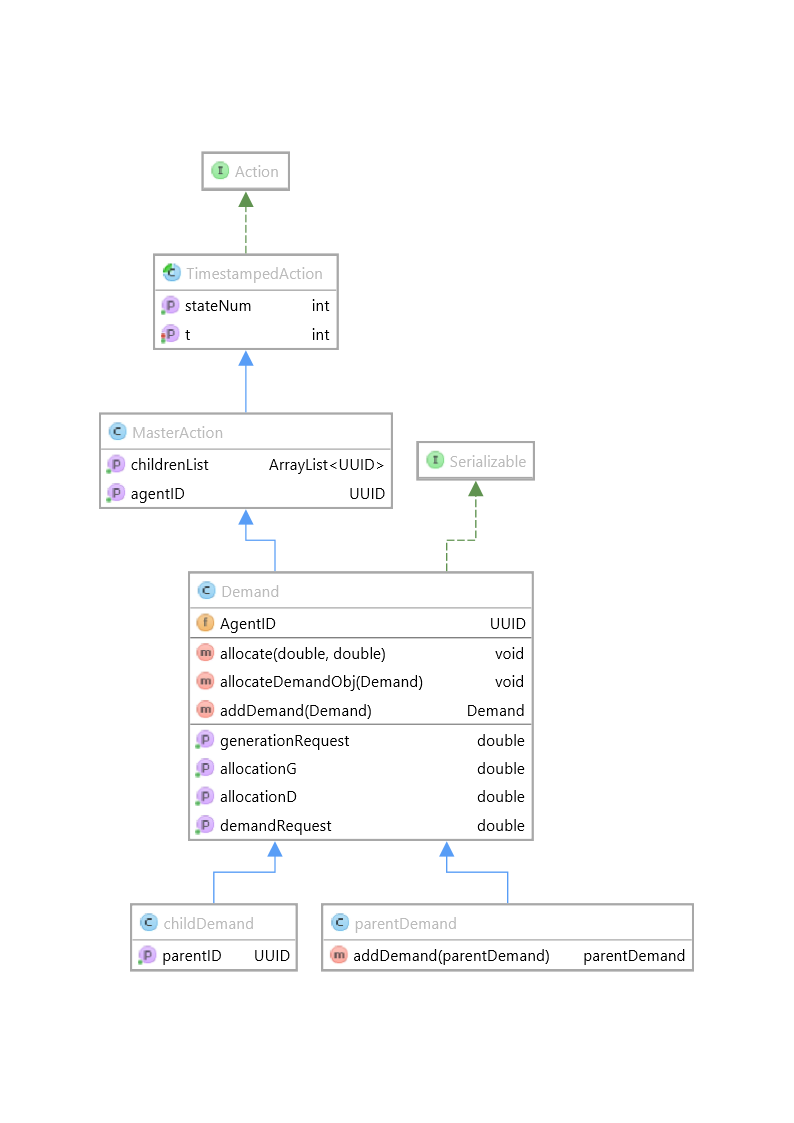
\includegraphics[scale=0.5]{Images/ActionUML.png}
	\caption{Actions UML Diagram}
	\label{fig:ActionUML}
\end{figure}

\subsection*{Action Handlers} % (fold)
To enable the Environment to be able to process the Action requests, Action Handlers need to be created to tell the simulation how to deal with Actions from Agents.

\begin{figure}[!h]
	\centering
	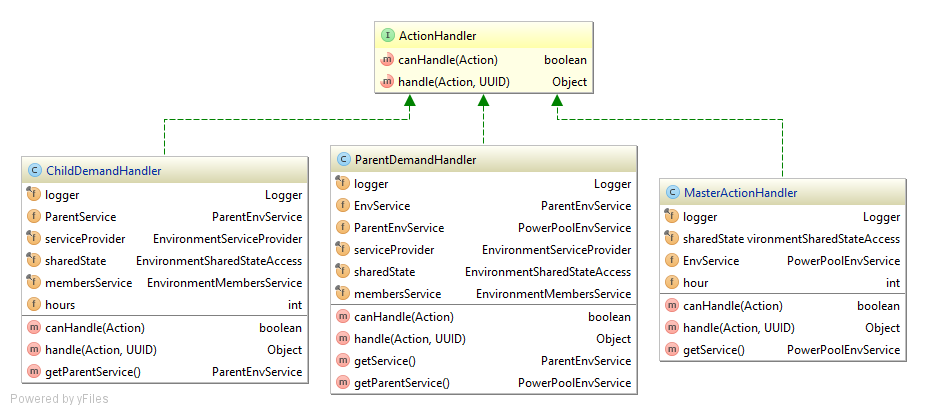
\includegraphics[scale=0.4]{Images/ActionHandlerUML.png}
	\caption{Action Handler UML Diagram}
	\label{fig:ActionHandlerUML}
\end{figure}
% subsubsection subsubsection_name (end)

\subsection*{Simulation}


\section*{Issues}
Out of order parallel execution meant that Agents need to submit their individual Demands to the SharedState, and have that summed at the end of each timestep. It is not possible to sum the Demands on the fly.

Being new to both Java and Presage presented problems of its own. It was difficult to understand how simulations could be run and therefore create our own.

One action per time step meant that it takes 4 time steps to simulate one round of request and appropriation of electricity. It would therefore take 24*4 time steps to simulate a full day of requests and appropriation.

% !TEX root = ../main.tex
\chapter{Testing}
\label{Testing}

The final product of this project should be a realistic simulation of a Decentralised Community Energy System. To produce the simulation, each of the following features will be tested to ensure they work individually and together:

\begin{itemize}
\item A network of Agents able to trade electricity with each other.
\item Agents are able to utilise energy. The amount of energy utilised can be pre-determined manually by an operator of the simulation or automatically with an algorithm.
\item Agents are able to generate an amount of energy corresponding to a pre-allocated fixed output, or an amount based on their assigned Generation Profiles.
\item Each Agent is able to utilise and generate electricity at the same time.
\end{itemize}

Due to time constraints, unit testing was not implemented. A series of tests was done manually by exporting the data using Excel to prove that the simulator was working as inteneded. The testing has been outlined in the sections below. Each of the tests below has been conducted for the following simulation cases:

\begin{itemize}
	\item 1 Supervisor, 1 Virtual Agent and 1 Agent
	\item 1 Supervisor, 2 Virtual Agent and 2 Agents (Each Virtual Agent connected to 1 Agent)
	\item 1 Supervisor, 2 Virtual Agents and 4 Agents (Each Virtual Agent connected to 2 Agents)
	\item 1 Supervisor, 5 Virtual Agents and 25 Agents (Each Virtual Agent connected to 5 Agents)
\end{itemize}

\section*{Contribution to Pool} % (fold)
To test that Agents are able to contribute to the Common Pool, the individual Demand and Generation request of each Agent was recorded in a CSV file. The allocations in the CSV file was summed and compared to that of the computed Global Demand and Generation request.

An example can be seen in \ref{fig:test1} of testing the contribution of 25 Agents during hour 23 of a simulation

\begin{figure}[h!]
	\centering
	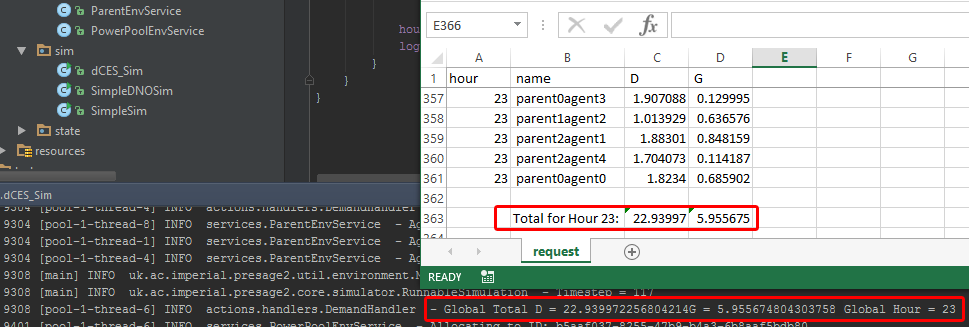
\includegraphics[scale=0.4]{Images/test-contribution.png}
	\caption{Testing the contribution at hour 23 of the simulation for 25 Agents}
	\label{fig:test1}
\end{figure}

\section*{Correct Allocation}
When the global aggregated Generation requests exceed the global aggregated Demand requests, all Agents are expected to receive their requests. Globally, Generation is curtailed to not exceed total Demand Request. Generation is curtailed proportionally for everyone. In this case, we should expect all Agents to be allocated less Generation than they have requested, and all Agents to be allocated their Demand requests. \\

An example of this test can be seen in \ref{fig:test2}. \\

\begin{figure}[h!]
	\centering
	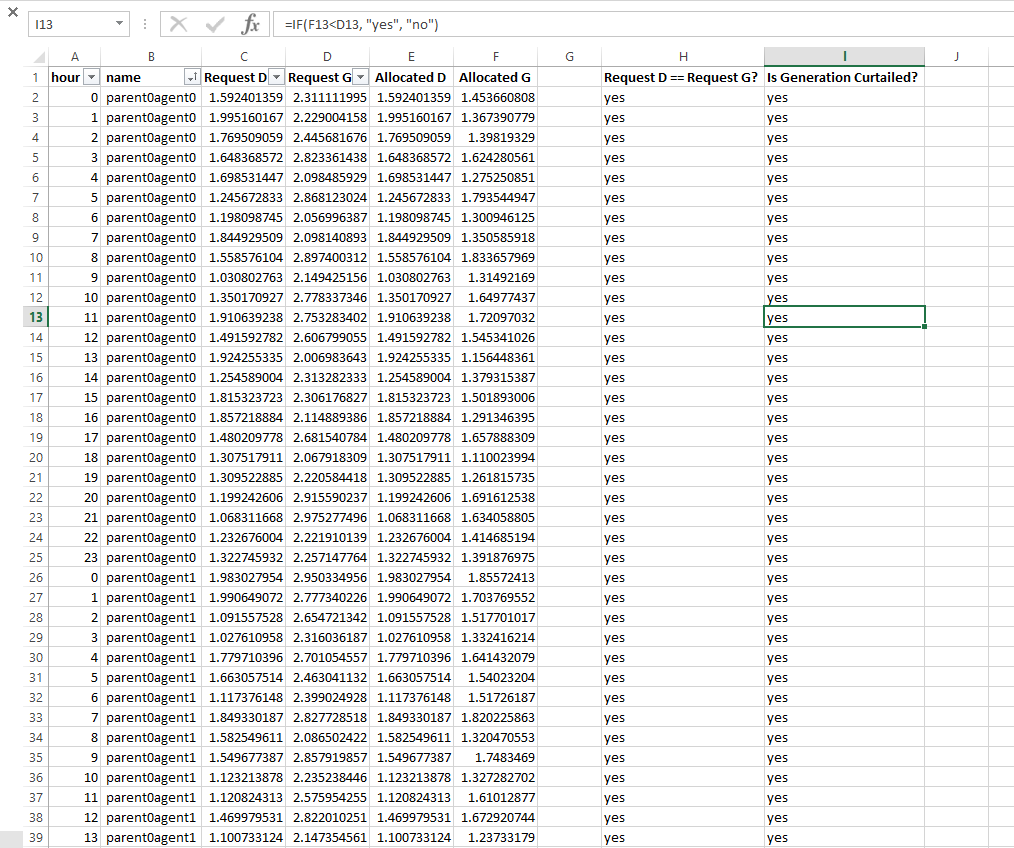
\includegraphics[scale=0.4]{Images/test-allocation1.png}
	\caption{Testing the allocation of 25 Agents when total Generation Request Exceeds total Demand Request}
	\label{fig:test2}
\end{figure}

When the global aggregated Demand request exceed the global Demand request, the fair allocation method will need to be used. For testing this, we need to ensure the following:

\begin{itemize}
	\item Allocated Demand is equal to Allocated Generation
	\item Allocated Generation is equal to Generation request
	\item Allocation proportion is correct
	\item Borda ranking is correct for each of the canons
	\item Borda voting by the Agents are correct
	\item Borda voting is taken into consideration in the next round
\end{itemize}

To be continued...

% section section_name (end)
%If data is available for the potential customers in Rugaragara, the simulation could be used in %conjunction with the feasibility study
% !TEX root = ../main.tex
\chapter{Results}
\label{Results}

\section*{Simulating over 24 hours}
Five clusters of 5 Prosumer Agents (25 Prosumer Agents, 5 Virtual Agents and 1 Supervisor Agents) were simulated over 24 hours. Each cluster had 2 Prosumers generating using Wind Turbines and 3 Prosumers generating using Photovoltaic cells. With no data about the economic output or social utility of the individual households in Rugaragara being available, the data had to be generated for the simulation. All Prosumer Agents were initialised with a random \textit{Productivity} rating and a random \textit{Social Utility} representing a household's hourly contribution to the economic or social development of the local community.

As expected, as long as there was some generation, all Prosumer Agents would receive some electricity. At no point in the simulation was there no electricity being received by the Prosumer Agents who were not generating at the time (solar powered Prosumers during the night). The general trend was that an Agent which was judged to have contributed more (under the \textit{Rescher's Canons of Distributive Justice}) would receive more allocation when Demand outstrips Generation, representing in a higher average satisfaction. As an example, the contribution according to the \textit{Rescher's Canon of Distributive Justice} of three of the Prosumers in \textit{Cluste0} has been included in table \ref{tab:cluster0}. In this example, it can be observed that the most satisfied \textit{Agent3} is contributing more than the least satisfied \textit{Agent0} across the board while maintaining a slightly smaller amount of requests over the simulated 24 hour period. 

\begin{table}[h]
\centering
	\caption{Prosumer Agent contribution data for Agent 0,1,3 in Cluster0}
	\label{tab:cluster0}
	\resizebox{\textwidth}{!}{%
	\begin{tabular}{llllll}
	\hline
	Agent & \begin{tabular}[c]{@{}l@{}}Average\\ Satisfaction\end{tabular} & \begin{tabular}[c]{@{}l@{}}Average \\ Request\end{tabular} & \begin{tabular}[c]{@{}l@{}}Average \\ Contribution\end{tabular} & \begin{tabular}[c]{@{}l@{}}Average\\ Productivity\end{tabular} & \begin{tabular}[c]{@{}l@{}}Social \\ Utility\end{tabular} \\ \hline
	0     & 0.712                                                          & 1.575                                                      & 2.214                                                           & 1.750                                                          & 1.667                                                     \\
	3     & 0.676                                                          & 1.577                                                      & 0.379                                                           & 1.958                                                          & 1.875                                                     \\
	1     & 0.770                                                          & 1.575                                                      & 2.213                                                           & 2.208                                                          & 2.167                                                     \\ \hline
	\end{tabular}
	}
\end{table}

It is interesting to find that Agents can sometimes receive more than what they have requested, resulting in a satisfaction rating that is above 1 (see table \ref{tab:SatisfactionMoreThanOne}). Opportunities such as these arise due to the holonic nature of the system, as the Supervisor Agent allocates fairly to the Virtual Agents. If as a cluster, it is contributing more than the other clusters, then at the Supervisor Allocation stage, this particular cluster will be allocated more energy. If an Agent within that Cluster is contributing more, then that Agent will be allocated more of an already big pool, which can lead to allocating more energy than is requested by the Agent. Take the cases of Clusters 2 and 3, which both have had multiple occurences of Agents being allocated more than requested; these clusters have had an above average contribution to the common pool which can be seen in table \ref{tab:ClusterRank}, and as a result have the two highest average satisfaction ratings. 

\begin{table}[h]
\centering
\caption{Occurences of when Agents are allocated more than requested}
\label{tab:SatisfactionMoreThanOne}
\resizebox{\textwidth}{!}{%
\begin{tabular}{@{}ccccccccc@{}}
\toprule
Hour & Agent          & \begin{tabular}[c]{@{}c@{}}Requested\\ Demand\end{tabular} & \begin{tabular}[c]{@{}c@{}}Requested\\ Generation\end{tabular} & Productivity & \begin{tabular}[c]{@{}c@{}}Social\\ Utility\end{tabular} & \begin{tabular}[c]{@{}c@{}}Allocated\\ Demand\end{tabular} & \begin{tabular}[c]{@{}c@{}}Allocated\\ Generation\end{tabular} & Satisfaction \\ \midrule
14   & Cluster1Agent4 & 1.472                                                      & 1.014                                                          & 3.000        & 3.000                                                    & 1.574                                                      & 1.014                                                          & 1.069        \\
22   & Cluster2Agent0 & 1.213                                                      & 2.367                                                          & 2.000        & 4.000                                                    & 1.282                                                      & 2.367                                                          & 1.057        \\
22   & Cluster2Agent1 & 1.213                                                      & 2.378                                                          & 4.000        & 0.000                                                    & 1.360                                                      & 2.378                                                          & 1.121        \\
22   & Cluster3Agent3 & 1.215                                                      & 0.000                                                          & 4.000        & 3.000                                                    & 1.275                                                      & 0.000                                                          & 1.049        \\
22   & Cluster3Agent4 & 1.215                                                      & 0.000                                                          & 2.000        & 1.000                                                    & 1.229                                                      & 0.000                                                          & 1.012        \\
14   & Cluster4Agent1 & 1.473                                                      & 1.712                                                          & 4.000        & 2.000                                                    & 1.877                                                      & 1.712                                                          & 1.275        \\ \bottomrule
\end{tabular}
}
\end{table}


\begin{table}[h]
\centering
\caption{Cluster contributions}
\label{tab:ClusterContributions}
\resizebox{\textwidth}{!}{%
\begin{tabular}{@{}llllll@{}}
\toprule
\multicolumn{1}{c}{Cluster} & \multicolumn{1}{c}{\begin{tabular}[c]{@{}c@{}}Average \\ Request\end{tabular}} & \multicolumn{1}{c}{\begin{tabular}[c]{@{}c@{}}Average \\ Contribution\end{tabular}} & \multicolumn{1}{c}{\begin{tabular}[c]{@{}c@{}}Average \\ Productivity\end{tabular}} & \multicolumn{1}{c}{\begin{tabular}[c]{@{}c@{}}Social \\ Utility\end{tabular}} & \multicolumn{1}{c}{\begin{tabular}[c]{@{}c@{}}Average \\ Satisfaction\end{tabular}} \\ \midrule
Cluster0 & 1.576 & 1.113 & 1.967 & 2.075 & 0.715 \\
Cluster1 & 1.575 & 1.113 & 1.658 & 2.092 & 0.724 \\
Cluster2 & 1.575 & 1.114 & 2.058 & 2.067 & 0.762 \\
Cluster3 & 1.575 & 1.113 & 2.175 & 2.125 & 0.800 \\
Cluster4 & 1.575 & 1.113 & 2.142 & 2.050 & 0.715 \\ \bottomrule
\end{tabular}
}
\end{table}

\begin{table}[h]
\centering
\caption{Ranked cluster contributions using the data from table \ref{tab:ClusterContributions}}
\label{tab:ClusterRank}
\begin{tabular}{@{}lllllll@{}}
\toprule
\multicolumn{1}{c}{Cluster} & \multicolumn{1}{c}{\begin{tabular}[c]{@{}c@{}}Average \\ Request\end{tabular}} & \multicolumn{1}{c}{\begin{tabular}[c]{@{}c@{}}Average \\ Contribution\end{tabular}} & \multicolumn{1}{c}{\begin{tabular}[c]{@{}c@{}}Average \\ Productivity\end{tabular}} & \multicolumn{1}{c}{\begin{tabular}[c]{@{}c@{}}Social \\ Utility\end{tabular}} & \multicolumn{1}{c}{\begin{tabular}[c]{@{}c@{}}Average \\ Ranking\end{tabular}} & \multicolumn{1}{c}{\begin{tabular}[c]{@{}c@{}}Average \\ Satisfaction\end{tabular}} \\ \midrule
Cluster0                    & 5                                                                              & 4                                                                                   & 4                                                                                   & 3                                                                             & 4                                                                              & 0.715                                                                               \\
Cluster1                    & 3                                                                              & 3                                                                                   & 5                                                                                   & 2                                                                             & 3.25                                                                           & 0.724                                                                               \\
Cluster2                    & 2                                                                              & 1                                                                                   & 3                                                                                   & 4                                                                             & 2.5                                                                            & 0.762                                                                               \\
Cluster3                    & 1                                                                              & 2                                                                                   & 1                                                                                   & 1                                                                             & 1.25                                                                           & 0.800                                                                               \\
Cluster4                    & 4                                                                              & 5                                                                                   & 2                                                                                   & 5                                                                             & 4                                                                              & 0.715                                                                               \\ \bottomrule
\end{tabular}
\end{table}
% !TEX root = ./main.tex
\chapter{Evaluation}
\label{Evaluation}
% !TEX root = ../main.tex
\chapter{Conclusion}
\label{Conclusions}

Since October, an attempt has been made to understand the concept of a Common Pool Resource, and how electricity can be a form of a Common Pool Resource for remote communities in developing countries. An attempt has been made on building a simulator of a Decentralised Community Energy System in developing countries, which can self-organise and fairly allocate electricity to end-users. The testing and results shows that the attempt has been successful in the following:
\begin{itemize}
	\item Incorporating multiple forms of generation, by allowing generation profiles to be imported in the form of CSV files
	\item Incorporating realistic Generator Models by using measured data
	\item Creating a self-organising holonic system which is also able to allocate available power fairly to all system participants
\end{itemize}

However, there were also a number of features that have could have been implemented to make the model potentially more realistic:
\begin{itemize}
	\item Cheating and Selfishness - The model that has been implemented assumes all parties participating in the micro-grid will provide all of their generation and only appropriate their allocated amount from the system. However, in the real world, people will be selfish and attempt to cheat to benefit themselves  
	\item Non-renewable sources of generation - Non-renewable sources of energy have not been included in this model, as they have a fuel cost, which is difficult to model, and also make it difficult to allocate fairly. 
	\item Cost of the system - In reality, a micro-grid costs money to set-up and maintain and no conductor is completely efficient, leading to losses in the cables, and thus additional costs. None of these have been modelled.
\end{itemize}

% \section{}

\section*{Potential Applications}
One obvious use case is the feasibility study of the Rugaragara Falls micro-grid. In the immediate future, it is hoped that this tool could be used to aid the feasibility study of the micro-grid to be implemented in Rugaragara Falls. Aside from modeling small scale community micro-grids, the model can also be scaled up to model country level smart grids once cable losses, reactive power flow have been incorporated into the simulation. 
This Simulator of a Decentralised Community Energy System can be further developed with more features to explore possible utilisation patterns within rural communities, and also explore controls for regulating the use of electricity in developed countries. 
% !TEX root = ./main.tex
\chapter{Further Work}
\label{Further Work}

So far, the works carried out will be only be applicable for one community in rural Rwanda. It is hoped that work will be carried out to make this applicable to other communities by including more generation types such as biogas, and more types of appliances owned by each house.

In the immediate future, it is hoped that this tool could be used to aid the feasibility study of the Micro-Grid to be implemented in Rugaragara Falls. Should there be time, an energy trading platform will be designed and built based on the model created in this project to provide adequate electricity access to all members of the community. However, the energy trading platform would require a different design and implementation scheme which is not included in this report.

The sections below outlines the various properties each Agent must be able to take and how they could be implemented for the simulation scenario of rural communities in Rwanda. All of the properties must be allowed to exist on the same Agent during simulation.

In addition, the e.quinox Micro Grid is currently undergoing feasibility studies. If time allows, a system could be designed and built for the Micro Grid to allow the trading of electricity between households to guarantee electricity supply for when it is needed. This system however will have a completely different set of requirements, which will be drawn up after the completion of this project.

Consider Diesel Generators' costs 
Consider satisfaction of individual agents for them to partake in this
% !TEX root = ./main.tex
\chapter{User Guide}
\label{Guide}

%\chapter{A Chapter of Examples}
\label{chapter1}

\section{A Table}

\begin{table}[h]
\centering
\begin{tabular}{rcc}
\toprule \emph{Feature} & \textsc{Misuse-based} &
\textsc{Anomaly-based}\\
    
\midrule Modeled activity: & Malicious & Normal\\
Detection method: & Matching & Deviation\\
Threats detected: & Known & Any\\
False negatives: & High & Low\\
False positives: & Low & High\\
Maintenance cost: & High & Low\\
Attack desc.: & Accurate & Absent\\
System design: & Easy & Difficult\\
\bottomrule
\end{tabular}
\caption[Duality between misuse- and anomaly-based intrusion detection techniques.]{Duality between misuse- and anomaly-based intrusion detection techniques. Note that, an anomaly-based \ac{IDS} can detect ``Any'' threat, under the assumption that an attack always generates a deviation in the modeled activity.}
\label{tab:misuse-vs-anomaly}
\end{table}

%------------------------------------------------

\section{Code}

\begin{pseudoc}[Caption Here]
  /* ... */ cd['<'] = {0.1, 0.11} cd['a'] = {0.01, 0.2} cd['b'] =
  {0.13, 0.23} /* ... */

  b = decode(arg3_value);
  
  if ( !(cd['c'][0] < count('c', b) < cd['c'][1]) ||\
       !(cd['<'][0] < count('<', b) < cd['<'][1]) ||\
       ... || ...)  fire_alert("Anomalous content detected!");
  /* ... */
\end{pseudoc}

% \begin{pseudoc}[Caption]
%   Agents submit Demand and Generation Requests to Virtual Agents
%   Virtual Agents submit Demand and Generation Requests to Supervisor
%   Supervisor determines amount of power available
%   Supervisor makes a provision of power to Virtual Agents
%   Virtual Agents makes a provision to Agents
% \end{pseudoc}

%------------------------------------------------

\section{A Sideways Table}

\clearpage
\begin{sidewaystable}
\renewcommand{\arraystretch}{1.5} \centering
\begin{tabular}{rcccccc}
\toprule \textsc{Approach} & \textsc{Time} & \textsc{Header} &
\textsc{Payload} & \textsc{Stochastic} & \textsc{Determ.} & \textsc{Clustering}\\
\midrule brea & & $\bullet$ & & & & $\bullet$ \\
a & & $\bullet$ & $\bullet$ & $\bullet$ & & \\
b & & $\bullet$ & & $\bullet$ & $\bullet$ & \\
c & & & $\bullet$ & & & $\bullet$ \\
d & $\bullet$ & & $\bullet$ & & $\bullet$ & \\
e & & $\bullet$ & $\bullet$ & & & $\bullet$ \\
f & & & $\bullet$ & $\bullet$ & & \\
g & & $\bullet$ & $\bullet$ & & & $\bullet$ \\
h & & $\bullet$ & $\bullet$ & & & $\bullet$ \\
i & & & $\bullet$ & $\bullet$ & & \\
\bottomrule
\end{tabular}
\caption{Taxonomy of the selected state of the art approaches for network-based anomaly detection.}
\label{tab:network-sota-taxonomy}
\end{sidewaystable}
\clearpage

%------------------------------------------------

\section{A Figure}

\begin{figure}[h]
\centering
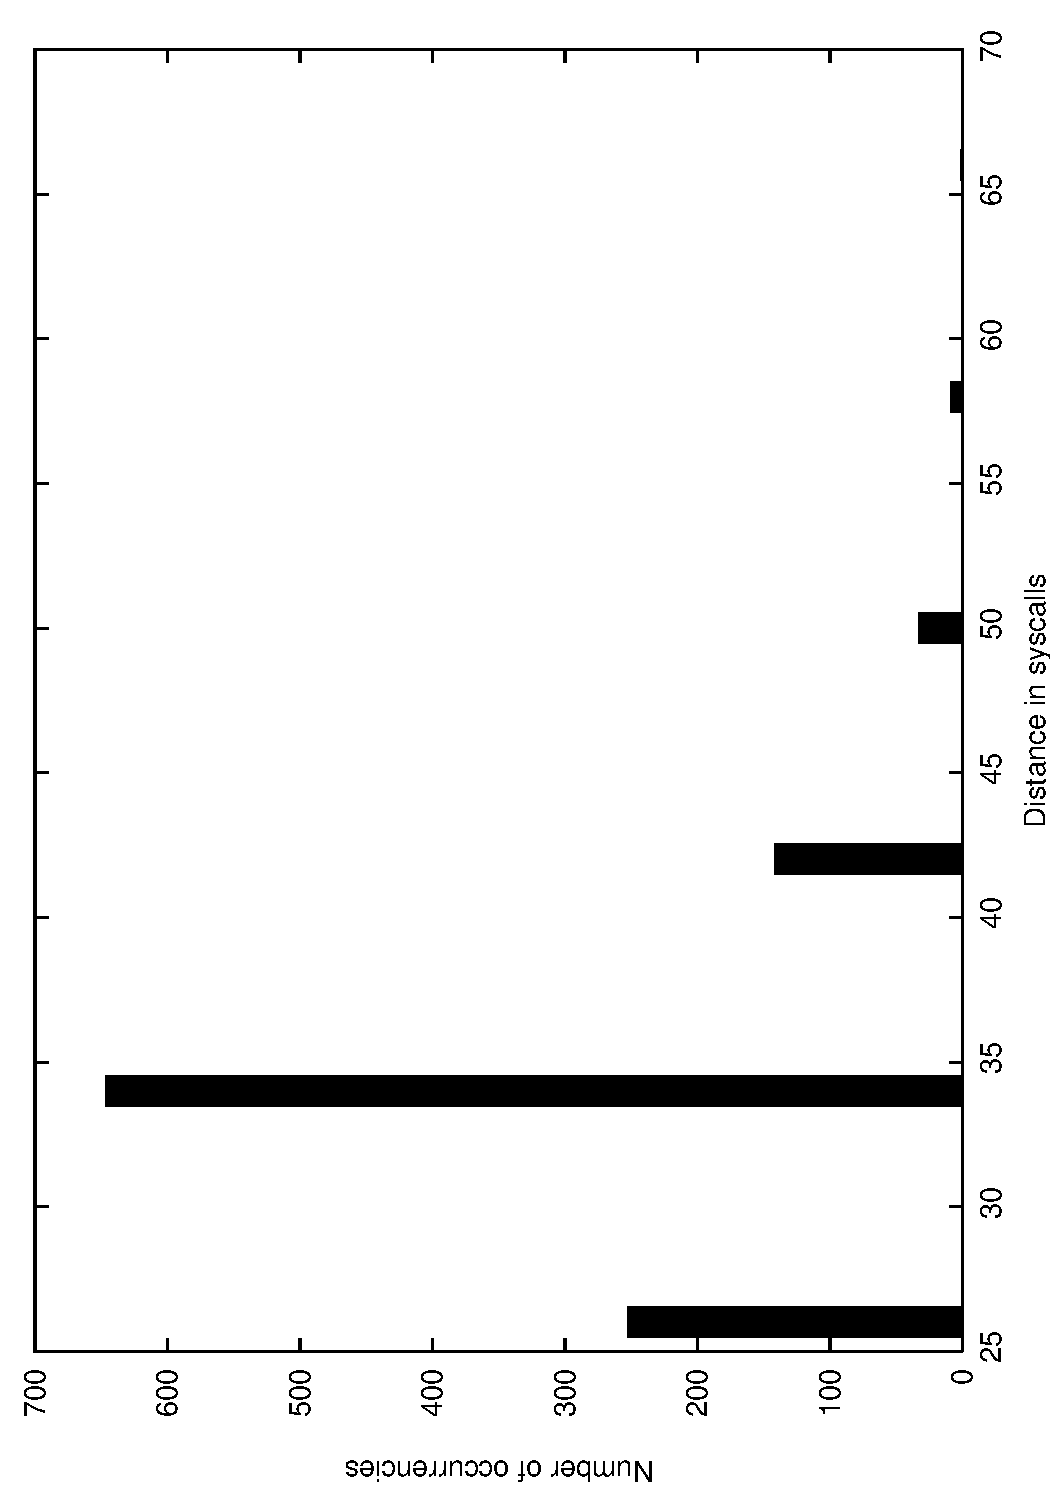
\includegraphics[angle=-90,width=.8\textwidth]{Figures/telnet.pdf}
\caption{\texttt{telnetd}: distribution of the number of other system calls among two \texttt{execve} system calls (i.e., distance between two consecutive \texttt{execve}).}
\label{fig:exectelnet}
\end{figure}

%------------------------------------------------

\section{Bulleted List}

\begin{itemize}
\item $O = $``Intrusion'', $\neg O =$``Non-intrusion'';
\item $A = $``Alert reported'', $\neg A =$``No alert reported''.
\end{itemize}

%------------------------------------------------

\section{Numbered List}

\begin{enumerate}
\item $O = $``Intrusion'', $\neg O =$``Non-intrusion'';
\item $A = $``Alert reported'', $\neg A =$``No alert reported''.
\end{enumerate}

%------------------------------------------------

\section{A Description}

\begin{description}
\item[Time] refers to the use of \emph{timestamp} information, extracted from network packets, to model normal packets. For example, normal packets may be modeled by their minimum and maximum inter-arrival time.
\item[Header] means that the \ac{TCP}\index{TCP} header is decoded and the fields are modeled. For example, normal packets may be modeled by the observed ports range.
\item[Payload] refers to the use of the payload, either at
\ac{IP}\index{IP} or \ac{TCP}\index{TCP} layer. For example, normal packets may be modeled by the most frequent byte in the observed payloads.
\item[Stochastic] means that stochastic techniques are exploited to create models. For example, the model of normal packets may be constructed by estimating the sample mean and variance of certain features (e.g., port number, content length).
\item[Deterministic] means that certain features are modeled following a deterministic approach. For example, normal packets may be only those containing a specified set of values for the \ac{TTL}\index{TTL} field.
\item[Clustering] refers to the use of clustering (and subsequent classification) techniques. For instance, payload byte vectors may be compressed using a \ac{SOM} where class of different packets will stimulate neighbor nodes.
\end{description}

%------------------------------------------------

\section{An Equation}

\begin{equation}
d_a(i,j) := \left\{
\begin{array}{lll}
K_a + \alpha_{a} \delta_{a}(i,j) & \mbox{if the elements are different} \\
0 & \mbox{otherwise}
\end{array}
\right.
\label{eq:distfunction}
\end{equation}

%------------------------------------------------

\section{A Theorem, Proposition \& Proof}

\begin{thm}
$a^2 + b^2 = c^2$
\end{thm}

\begin{prop}
$3 + 3 = 6$
\end{prop}

\begin{proof}
For any finite set $\{p_1,p_2,...,p_n\}$ of primes, consider $m = p_1p_2...p_n+1$. If $m$ is prime it is not in the set since $m > p_i$ for all $i$. If $m$ is not prime it has a prime divisor $p$. If $p$ is one of the $p_i$ then $p$ is a divisor of $p_1p_2...p_n$ and hence is a divisor of $(m - p_1p_2...p_n) = 1$, which is impossible; so $p$ is not in the set. Hence a finite set $\{p_1,p_2,...,p_n\}$ cannot be the collection of all primes.
\end{proof}

%------------------------------------------------

\section{Definition}

\begin{definition}[Anomaly-based \ac{IDS}]
An \emph{anomaly-based \ac{IDS}} is a type of \ac{IDS} that generate alerts $\mathbb{A}$ by relying on normal activity profiles.
\end{definition}

%------------------------------------------------

\section{A Remark}

\begin{rem}
Although the network stack implementation may vary from system to system (e.g., \textsf{Windows} and \textsf{Cisco} platforms have different implementation of \ac{TCP}).
\end{rem}

%------------------------------------------------

\section{An Example}

\begin{example}[Misuse \emph{vs.} Anomaly]\label{ex:misuse-vs-anomaly}
A misuse-based system $M$ and an anomaly-based system $A$ process the same log containing a full dump of the system calls invoked by the kernel of an audited machine. Log entries are in the form:

\begin{center}\small
\begin{verbatim} <function_name>(<arg1_value>, <arg2_value>, ...)
\end{verbatim}
\end{center}
\end{example}

%------------------------------------------------

\section{Note}

\begin{note}[Inspection layer]\label{note:network-stack-standardized}
Although the network stack implementation may vary from system to system (e.g., \textsf{Windows} and \textsf{Cisco} platforms have different implementation of \ac{TCP}), it is important to underline that the notion of IP, TCP, HTTP \emph{packet} is well defined in a system-agnostic way, while the notion of \emph{operating system activity} is rather vague and by no means standardized.
\end{note}
 % Include the first content chapter
 % Include the second content chapter
%\include{Chapters/chapter3} % Include the third content chapter

\backmatter

\chapterstyle{default} % Reset the chapter style back to the default used for non-content chapters

%----------------------------------------------------------------------------------------
%   BIBLIOGRAPHY
%----------------------------------------------------------------------------------------

\bibliographystyle{ieeetr} % Use the plainnat bibliography style

\bibliography{bibliography} % Use the bibliography.bib file as the source of references

%----------------------------------------------------------------------------------------
%   INDEX
%----------------------------------------------------------------------------------------

\printindex % Print the index

%----------------------------------------------------------------------------------------

\end{document}